\section{Concolic Execution vs.\ AFL}

We re-ran Problems 11, 12, 13, 14, 15 and 17 with our new concolic
fuzzer (5 minutes per problem) and compared it against the AFL results
from the previous lab. Figure~\ref{fig:conv} shows the convergence
curves of both strategies, and Figure~\ref{fig:bar} the final number of
unique error codes found.

\begin{figure}[H]
    \centering
    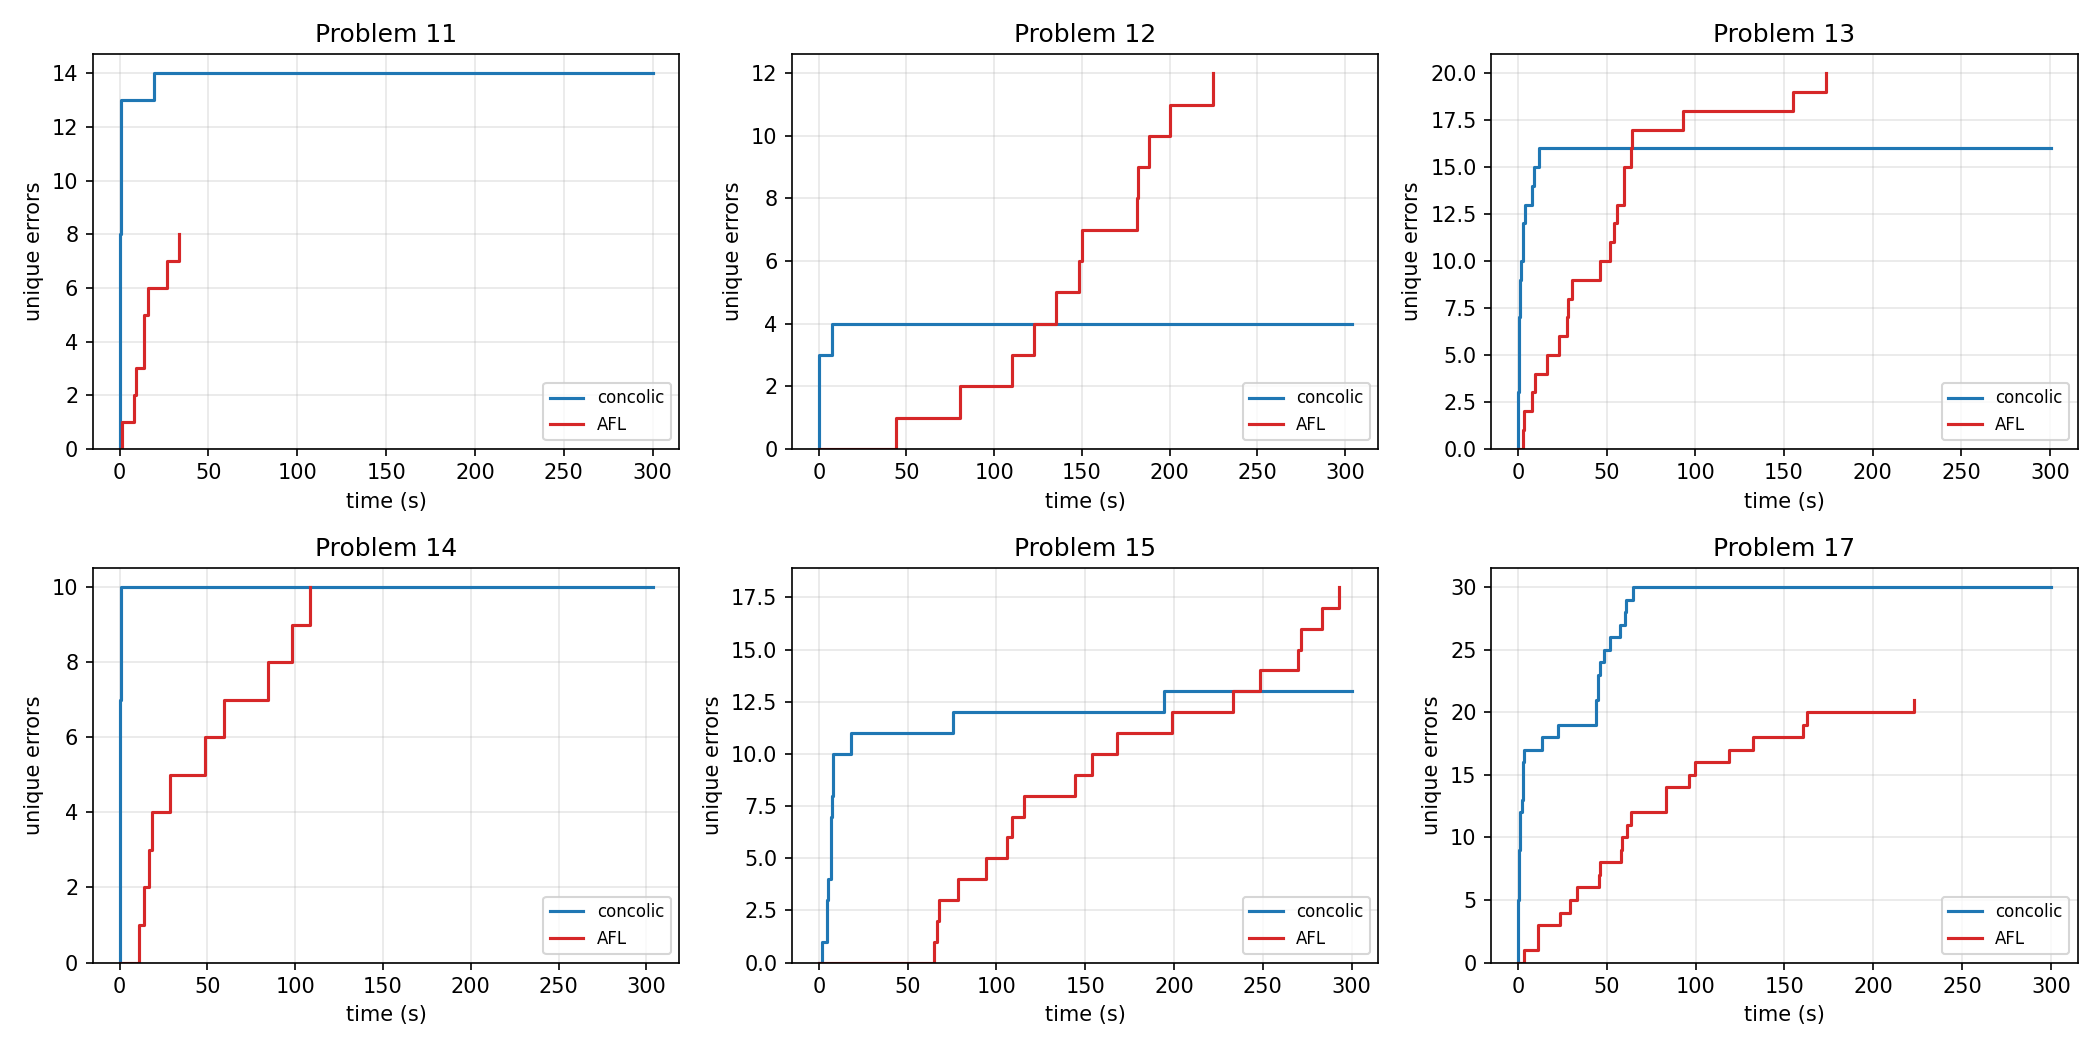
\includegraphics[width=\linewidth]{report/concolic_vs_afl_convergence.png}
    \caption{Unique error codes vs.\ time (5\,min budget) for the
    concolic fuzzer (blue) and AFL (red).}
    \label{fig:conv}
\end{figure}

\begin{figure}[H]
    \centering
    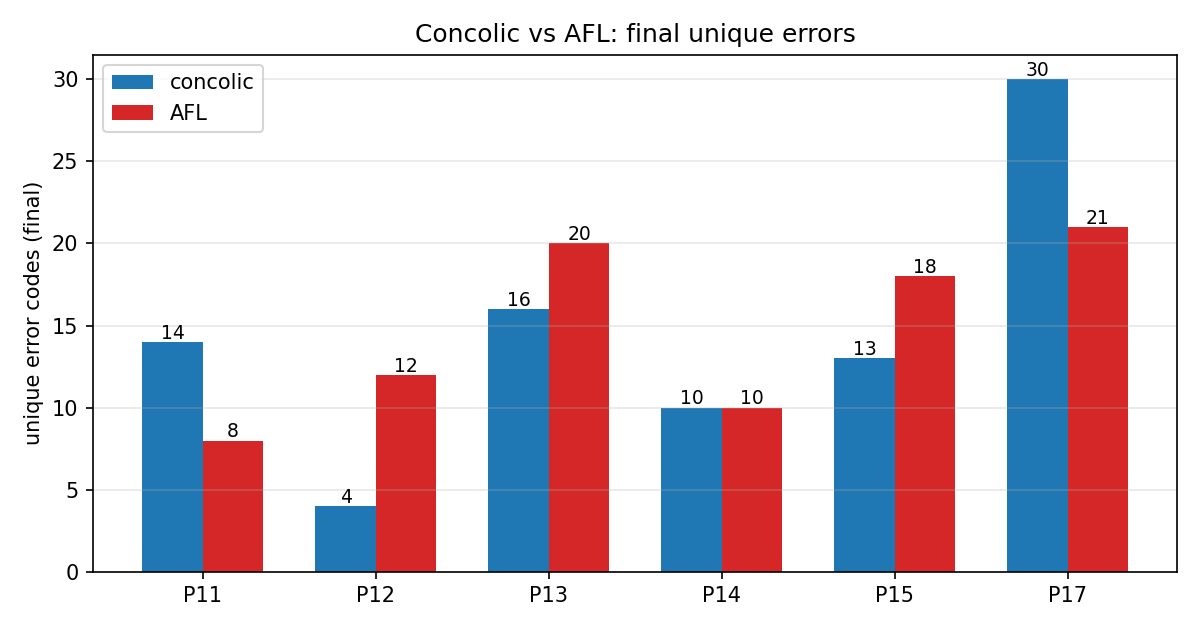
\includegraphics[width=0.85\linewidth]{report/concolic_vs_afl_bar.png}
    \caption{Final unique error counts after 5\,min.}
    \label{fig:bar}
\end{figure}

\paragraph{Findings.}
\begin{itemize}
    \item \textbf{Concolic wins on P11 and P17} (14 vs.\ 8, and 30 vs.\
    21). Both contain branches with strict numeric guards that AFL only
    breaks through by chance; the SMT solver flips them deterministically
    on the first visit, so the concolic curve climbs sharply in the first
    few seconds and then plateaus as new constraints become harder.
    \item \textbf{Tie on P14} (10 vs.\ 10). Both strategies appear to
    have exhausted the reachable error codes within the budget.
    \item \textbf{AFL wins on P12, P13 and P15.} On these problems the
    concolic fuzzer gets stuck early: P12 collapses at 4 errors because
    the solver-derived traces all share a common deep prefix, so the
    queue dries up and the random fallback rarely reaches new code.
    P13 and P15 show the same shape -- a fast initial burst (matching
    AFL's progress in the first $\sim$30\,s) followed by a long flat
    tail where AFL keeps discovering new errors through coverage-guided
    mutation.
    \item \textbf{Shape of the curves.} The concolic curves are
    step-like with most of the gain in the first 10--30\,s, after which
    progress stops almost completely. AFL converges more gradually and
    is still finding new errors near the end of the budget on most
    problems; given more time it would likely keep improving, whereas
    the concolic fuzzer has effectively converged.
\end{itemize}

\paragraph{Which strategy is better?}
Neither dominates the other. The concolic fuzzer is the right tool when
the program is gated by tight equality/inequality constraints that
random mutation cannot satisfy (P11, P17): it reaches deep errors in
seconds. AFL is the better choice when the search space is wide and
the path constraints fan out, because its coverage feedback keeps
producing new inputs long after the solver-driven queue is empty (P12,
P13, P15). In practice the two are complementary: a hybrid that seeds
AFL with concolic-generated inputs (or runs concolic to break specific
hard branches AFL is stuck on) would very likely outperform either
strategy alone on all six problems.
